\subsubsection{Mechanism for scoring alpinists}
  
  Engineering tasks included in this module:
  \begin{enumerate*}
    \item The first step was find all the sizes of climbers and elements of field that essential for creating module. The size of the box for climbers is the same to the box for debris: 14.6 x 5.75 . The height of the border is about 30 cm. The parameters of the climber 11.6 x 2 x 3 cm. It's weight is approximately 10-20g .
    
    \item After that it was invented the image of the mechanism for scoring climbers into the box. The lever with a container for climbers turns around the axis, which is placed higher than the edge of the border. The container is closed by a cover with a latch, that is tied to the mount of the axis by thread. When the container overturns, the thread stretches and releases the latch. It allows to throw climbers vertically with high accuracy and prevent them from accidental falling out of the container during the movement.
    
    \item According to this idea it was created the model of the bucket in Creo Parametric. To prevent the servo from breaking down, it was provided a second lever opposite the bucket, that can be charged with contraweight. It was also created a blueprint of a bucket and a cover. These elements will be made of PET.
    
    \item Next, the first version of the module was assembled and tested. The latch for cover was working stable. However, after the implementation in real details it was acknowledged, that the module is quite bulky because of the lever for contraweight. So, there were held calculations of the moment on the servo to investigate whether it can operate without a countraweight or not.
    
    \item The module was tested. It worked, but it was too bulky ant took too much space in the robot. So it was decided to refuse this construction.
    
    \item It was decided to make next construction. There is a TETRIX aluminium tube that turn by servo in vertical plane (so that when servo turn tube fall on the top of button). At the end of tube there is U shaped profile. Through the tube and U shaped profile is axis where hang climbers. U-shaped profile dosen't allow climbers to fall during the robot's moving. Also there is a line fixed on the end of axis. The line reel by the second servo so axis move and climbers fall to shelter.
    \begin{figure}[h]
    	\begin{minipage}[h]{1\linewidth}
    		\center{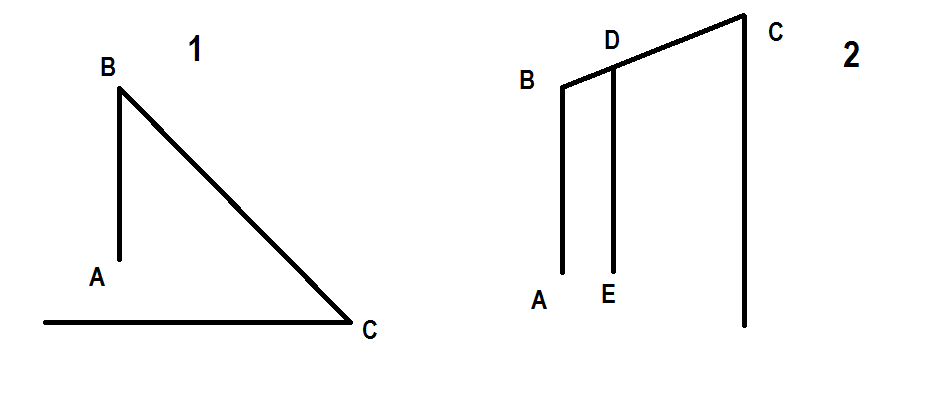
\includegraphics[scale = 0.4]{3Engineering/6Specifications_for_modules/alpinists/images/01}}
    		\caption{Mechanism for scoring climbers}
    	\end{minipage}
    \end{figure}
  
  \end{enumerate*}	
  
  
  